\documentclass[a4paper, 11pt]{article}

% Pacchetti necessari
\usepackage[utf8]{inputenc}
\usepackage[T1]{fontenc}
\usepackage[english]{babel}
\usepackage[left=2cm, right=2cm, top=2.5cm, bottom=2.5cm]{geometry}

\usepackage{graphicx} %for includegraphics

\usepackage{xcolor}
\definecolor{pastelblue}{RGB}{70,70,180}
\definecolor{pastelred}{RGB}{180,70,70}
\definecolor{orangeUSA}{RGB}{255, 112, 67}
\definecolor{lightorangeUSA}{RGB}{255, 151, 118}
\definecolor{matblue}{RGB}{0, 113.985, 188.955}
\definecolor{matred}{RGB}{216.75, 82.875, 24.99}
\definecolor{matyellow}{RGB}{236.895, 176.97, 31.875}

\usepackage{enumitem}
\setlist[description]{leftmargin=15mm}

\usepackage{titlesec}
\titleformat*{\section}{\large\bfseries\color{pastelred}}
\titlelabel{}


\usepackage{fontawesome}

\usepackage{hyperref}
\hypersetup{
    colorlinks = true,
    urlcolor=pastelblue,
}

% Definizioni personalizzate per le sezioni
\newcommand{\cvsection}[1]{\section*{#1}}
\newcommand{\cvsubsection}[1]{\subsection*{#1}}

% Inizio del documento
\begin{document}

% Informazioni personali
\begin{minipage}{0.2\textwidth}
    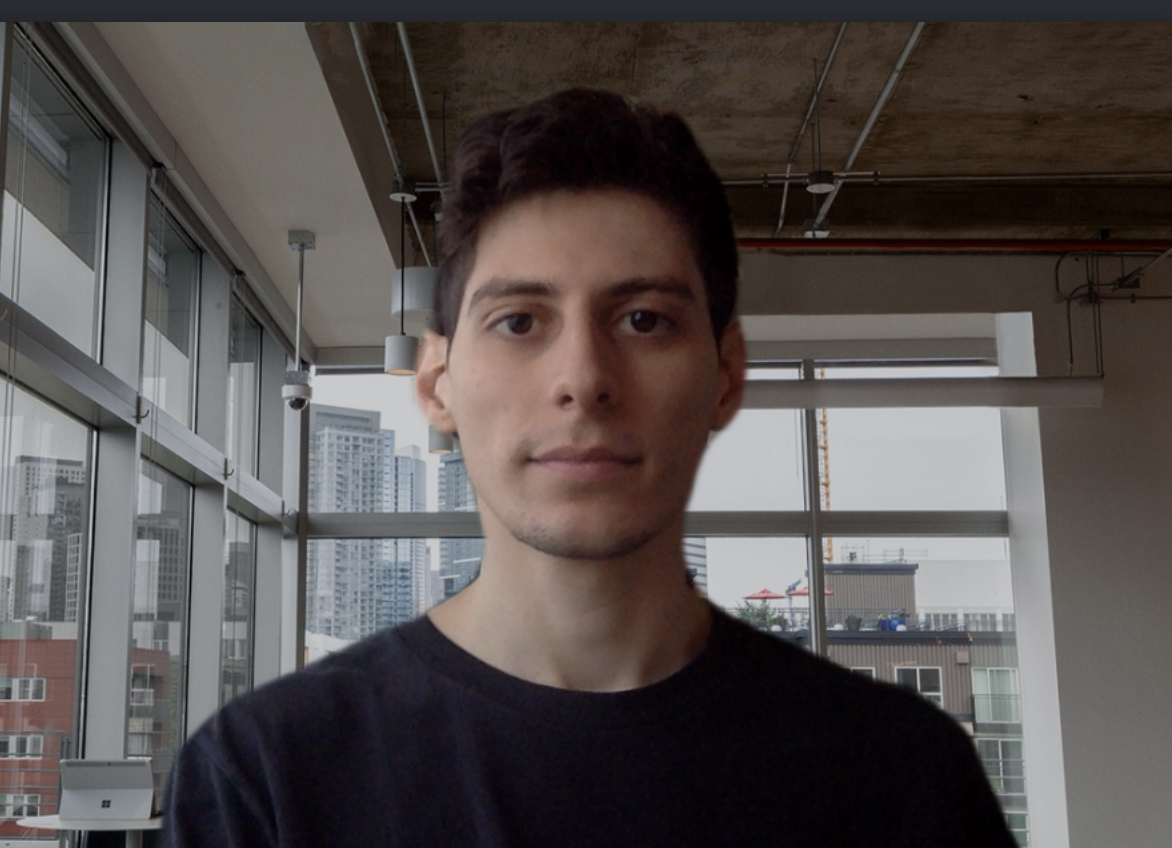
\includegraphics[scale=0.2]{images/fotoSkype.png}
\end{minipage}
%using minipage+center the sum fotopage + infopage/2 = textwidth/2
\begin{minipage}{0.6\textwidth}
    \begin{center}
        \textbf{\LARGE Antonio Minighin}
    \end{center}
    \begin{center}
        \faHome \ Padova, 35139, Italy \\
        \faMobile \ +39 329 3528187 \\
        \faPaperPlane \ \href{mailto://toto.minighin@gmail.com}{toto.minighin@gmail.com} \\
        \href{https://github.com/antomini}{\faGithub} \ | \
        \href{https://linkedin.com/in/antonio-minighin-b92074236}{\faLinkedinSquare}
    \end{center}
\end{minipage}


% Sezione: Formazione universitaria
\section*{ACADEMIC EDUCATION}
\begin{description}[leftmargin=5mm]
    \item \textbf{Master's Degree in Electronic Engineering 100/110}, Università degli Studi di Padova \hfill 2023
    \begin{description}
        \item[-] \href{https://thesis.unipd.it/handle/20.500.12608/48003}{Thesis}: PWM controller design with Zynq SoC, an embedded control system for switching mode power applications
        \item[-] Specialization: Analog and digital IC for processing and control systems
        %\item Courseworks: High-frequency matching networks, analog controller and filters, DSP techniques
    \end{description}
    \item \textbf{Bachelor's Degree in Electronic Engineering 87/110}, Università degli Studi di Padova \hfill 2019
    \begin{description}
        \item[-] Thesis: Sigma Delta ADC for audio applications, how to increase resolution using oversampling and modulation techniques
    \end{description}
\end{description}

\newcommand{\redminus}{\textcolor{matred}{\faMinus}}
\newcommand{\blueminus}{\textcolor{matblue}{\faMinus}}

\section*{MAIN EXAMS
            \hfill
            1CFU=8h LECTURES \hspace{1mm} | \hspace{1mm} 
            \textcolor{matred}{\faMinus \hspace{1mm} 9 CFU}
            \textcolor{matblue}{\faMinus \hspace{1mm} 6 CFU}
            }
\begin{minipage}[t]{0.45\textwidth}
    \begin{description}[leftmargin=5mm]
        \item[\redminus] Microelectronics
        \item[\redminus] Analog electronics
        \item[\blueminus] Analogue integrated circuit design
        \item[\blueminus] Integrated circuits for signal processing
        \item[\blueminus] Digital circuits design
        \item[\blueminus] Digital signal processing
        \item[\blueminus] Digital control
        \item[\redminus] Computer architectures
    \end{description}
\end{minipage}
\hfill
\begin{minipage}[t]{0.45\textwidth}
    \begin{description}[leftmargin=5mm]
        \item[\blueminus] Microcontrollers and DSP
        \item[\redminus] Industrial electronics 
        \item[\redminus] Power electronics
        \item[\redminus] Microwave devices
        \item[\redminus] Electronic measurements
        \item[\blueminus] Quality and reliability in electronics
        \item[\redminus] Economics and business organizations 
        \item[\redminus] Machine learning
    \end{description}
\end{minipage}

% Sezione: Esperienze lavorative
\section*{WORKING EXPERIENCE}
\begin{description}[leftmargin=5mm]
    \item \textbf{Internship at DAVE Embedded Systems}, Pordenone \hfill 6 months in 2022
    \begin{description}
        \item[-] Activity: Embedded system design using Zynq SoC
        \item[-] Project: FPGA based waveform generator for automatic power up test
    \end{description}
    \item \textbf{Internship at DAVE Embedded Systems}, Pordenone \hfill 3 months in 2018
    \begin{description}
        \item[-] Activity: Hardware acceleration using Zynq SoC
        \item[-] Project: High-level synthesis of computer vision algorithm using Pynq framework
    \end{description}
\end{description}

% Sezione: Competenze tecniche
\section{TECHNICAL SKILLS}
\subsection{System Design}
\begin{description}[leftmargin=5mm]
    \item[-] Good knowledge of HDL language for synthesis and functional verification of components on FPGA based devices. Design of processing pipeline and control interfaces targeting specific applications.
    \item[-] Good knowledge on programming and configuring embedded devices to reach SW and HW integration. Acceleration and safe execution of real-time and critical processes using interrupts and multiprocessing techniques.
    \item[-] Good knowledge of PCB realization based on specifications, such as signal integrity or thermal dissipation. Design of circuit for different solutions, like analog precise devices, high-speed digital interfaces and power converters.
    \item[-] Good knowledge of laboratory equipment for design verification, like oscilloscope, waveform generators, logic analyzers and debuggers.
\end{description}
\subsection{Programming}
\begin{description}[leftmargin=5mm]
    \item[- Languages:] VHDL, Verilog, Assembly, C/C++, Java, Python, Matlab.
    \item[- Devices:] AVR, ATmega, ARM Cortex-M/A, SAM3X, STM32F3, STM32F4, Artix-7, Zynq.
\end{description}

\subsection{Tools}
\begin{description}[leftmargin=5mm]
    \item[- CAD:] LTspice, KiCAD, Virtuoso, Design Vision, Vivado, Simulink.
    \item[- IDE:] Eclipse, Vitis, TrueStudio, Arduino.
    \item[- OS:] Windows, Ubuntu, macOS.
\end{description}

\section{SPOKEN LANGUAGES}
\begin{description}[leftmargin=5mm]
    \item[-Italian:] Native
    \item[-English:] B2 at Trinity College - ISE II certification
    % \item[-Spanish:] Basic understanding
\end{description}

\section{RESUME}
Studying electronic engineering was a straightforward decision driven by my passion about music, particularly electric guitar and electronic synthesizers.
Alongside the academic courses focused on designing analog and digital IC for processing and control systems, my interests fall on programmable embedded devices, like microcontrollers, FPGAs and CPU architectures.
I attended two internships at the DAVE embedded systems of Pordenone (Italy) to get in touch with real world applications and industry standard methodologies.
I worked with Zynq technology, an embedded solution for hardware design and software development suited for real-time operations and Linux based systems. 
With this technology, I managed to build a full-custom switching mode control system for power applications, by designing and testing components in a fully integrated environment.
Finally, I discussed the thesis on this project pointing out some topics, like the benefits of hardware parallelization for digital signal processing and the integration of hardware and software for real-time systems.
Now I'm looking for a place to start a career as electronic designer, preferably using embedded digital systems, where I can express creativity and apply knowledge to contribute on valuable projects.


% Fine del documento
\end{document}
